\documentclass[11pt,a4paper]{article}
\usepackage[utf8]{inputenc}
\usepackage[T1]{fontenc}
\usepackage[english]{babel}
\usepackage[a4paper,margin=2.5cm]{geometry}
\usepackage{graphicx}
\usepackage{subcaption}
\usepackage{tikz}
\usepackage{hyperref}
\usepackage{enumitem}
\usepackage{parskip}
\usepackage{float}
\usepackage{placeins}

% Limit image height for very tall mobile mockups
\newcommand{\maxgraph}[2][]{% width optional, height fixed to 0.4\textheight
  \includegraphics[#1,height=0.4\textheight,keepaspectratio]
  {#2}%
}

\title{WeatherNow Calendar Integration\\\large Portfolio Assignment 02: UI/UX Design}
\author{
  \begin{tabular}{ll}
    Pascal Putz & \href{mailto:pascal.putz@study.thws.de}{pascal.putz@study.thws.de} (5123135)\\
    Gunn Kataria & \href{mailto:gunn.kataria@study.thws.de}{gunn.kataria@study.thws.de} (9125072)\\
    Katrina Alex & \href{mailto:katrina.alex@study.thws.de}{katrina.alex@study.thws.de} (9125071)\\
    Manuel Stöth & \href{mailto:manuel.stoeth@study.thws.de}{manuel.stoeth@study.thws.de} (5123045)\\
    Marvin Kraus & \href{mailto:marvin.kraus@study.thws.de}{marvin.kraus@study.thws.de} (5123143)
  \end{tabular}
}
\date{May 2025}

\begin{document}

\maketitle
\tableofcontents

\newpage

\section{Summary of Requirements}
Based on our Requirements Document, WeatherNow Calendar Integration is a React.js web application that combines real-time weather data (via OpenWeatherMap API) with the user’s Google Calendar (via Google Calendar API) to suggest context-aware activities. It must:

\begin{itemize}[noitemsep]
  \item Display current weather and a 5-day forecast for any city or geolocation.
  \item Integrate Google Calendar to detect free/busy slots for scheduling suggestions.
  \item Recommend personalized indoor or outdoor activities according to weather conditions and user availability.
  \item Provide a toggle between light and dark themes and a unit switch (°C/\textdegree F).
  \item Ensure responsive design across devices with accessible navigation to Home, Forecast, and Calendar views.
  \item Handle errors gracefully, including invalid input, permission denials, and API failures.
\end{itemize}

\section{User Interface Design}
This section presents mid-fidelity desktop and mobile mockups for the key screens: Home, Forecast, and Calendar. Each view is shown in light and dark variants, with mobile versions demonstrating responsive stacking and touch improvements.

\subsection{Home Screen}
\FloatBarrier
\begin{figure}[H]
  \centering
  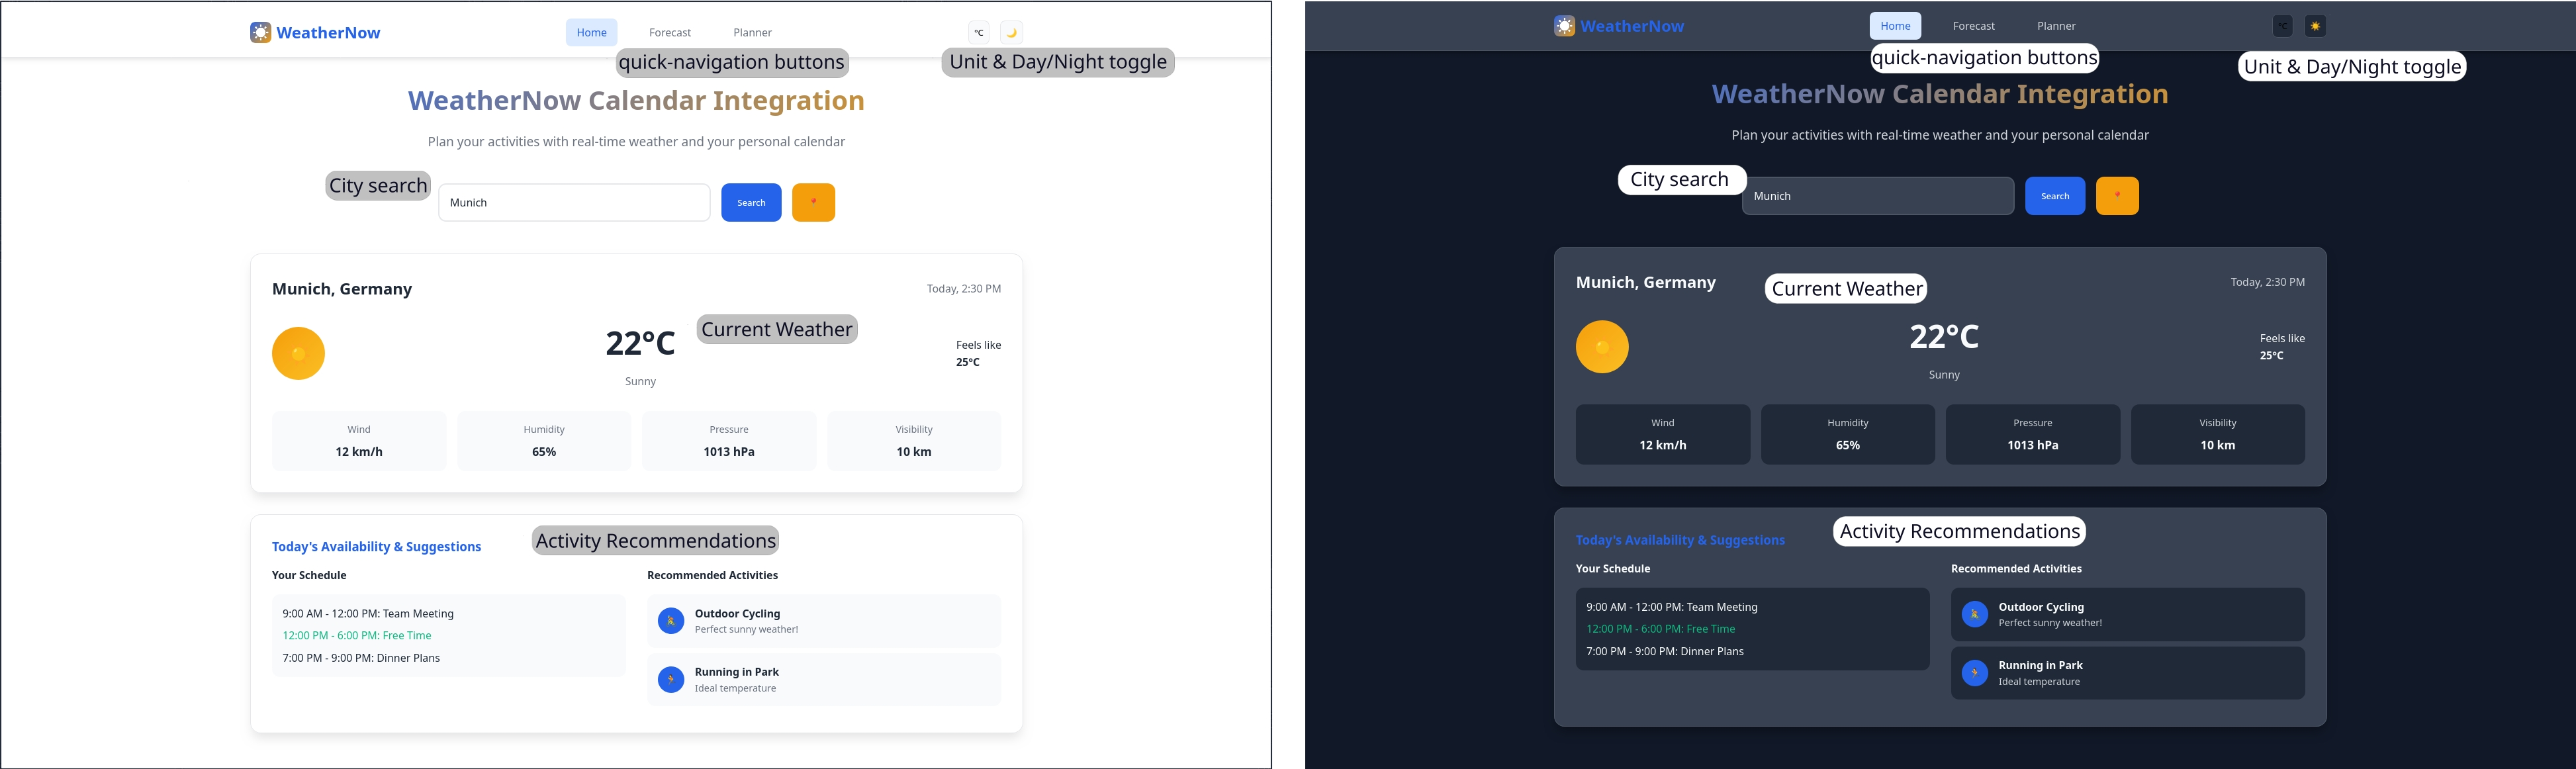
\includegraphics[width=\linewidth]{desktop_home_descripted.jpg}
  \caption{Home screen (desktop) with search, theme toggle, and summary of current weather and calendar suggestions.}
  \label{fig:home_desktop}
\end{figure}
\FloatBarrier

\subsection{Forecast Screen}
\FloatBarrier
\begin{figure}[H]
  \centering
    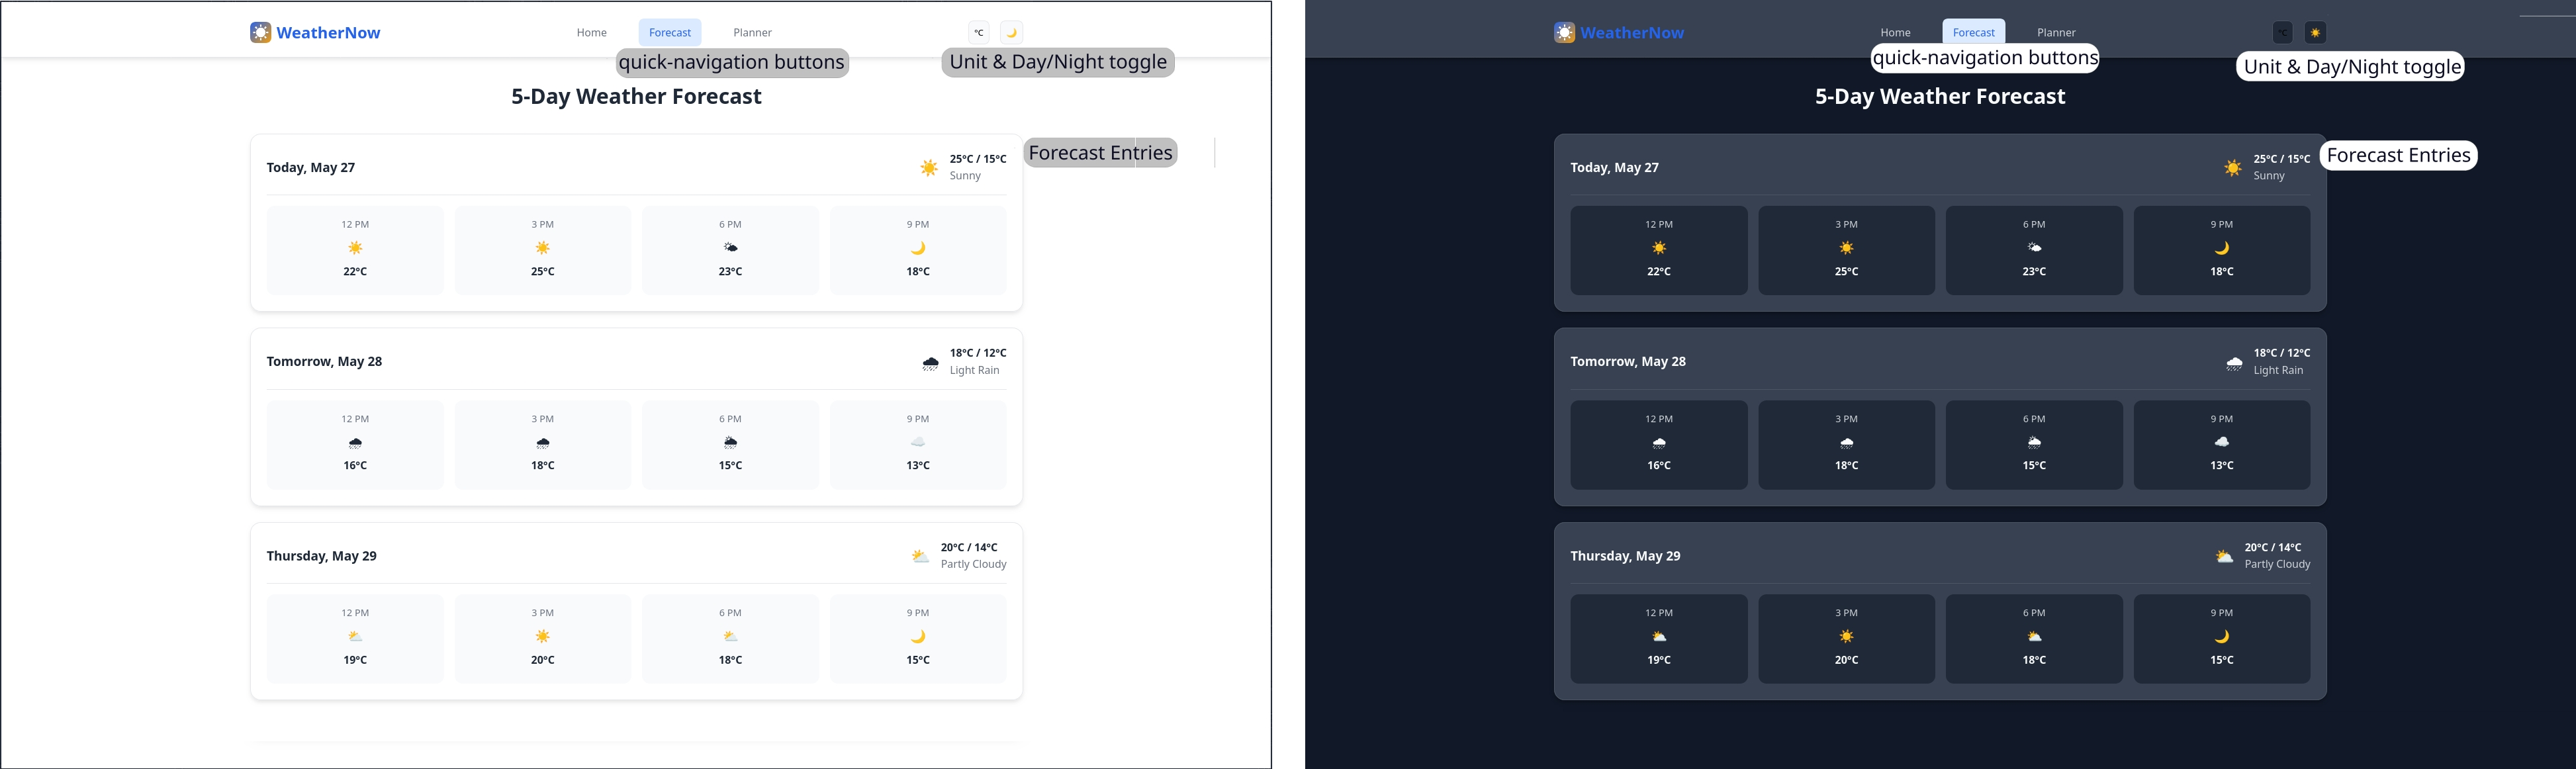
\includegraphics[width=\linewidth]{desktop_forecast_descripted.jpg}
  \caption{5-day weather forecast (desktop) with interval cards, icons, and summary metric.}
  \label{fig:forecast_desktop}
\end{figure}
\FloatBarrier


\subsection{Calendar \& Planner Screen}
\FloatBarrier
\begin{figure}[H]
  \centering
  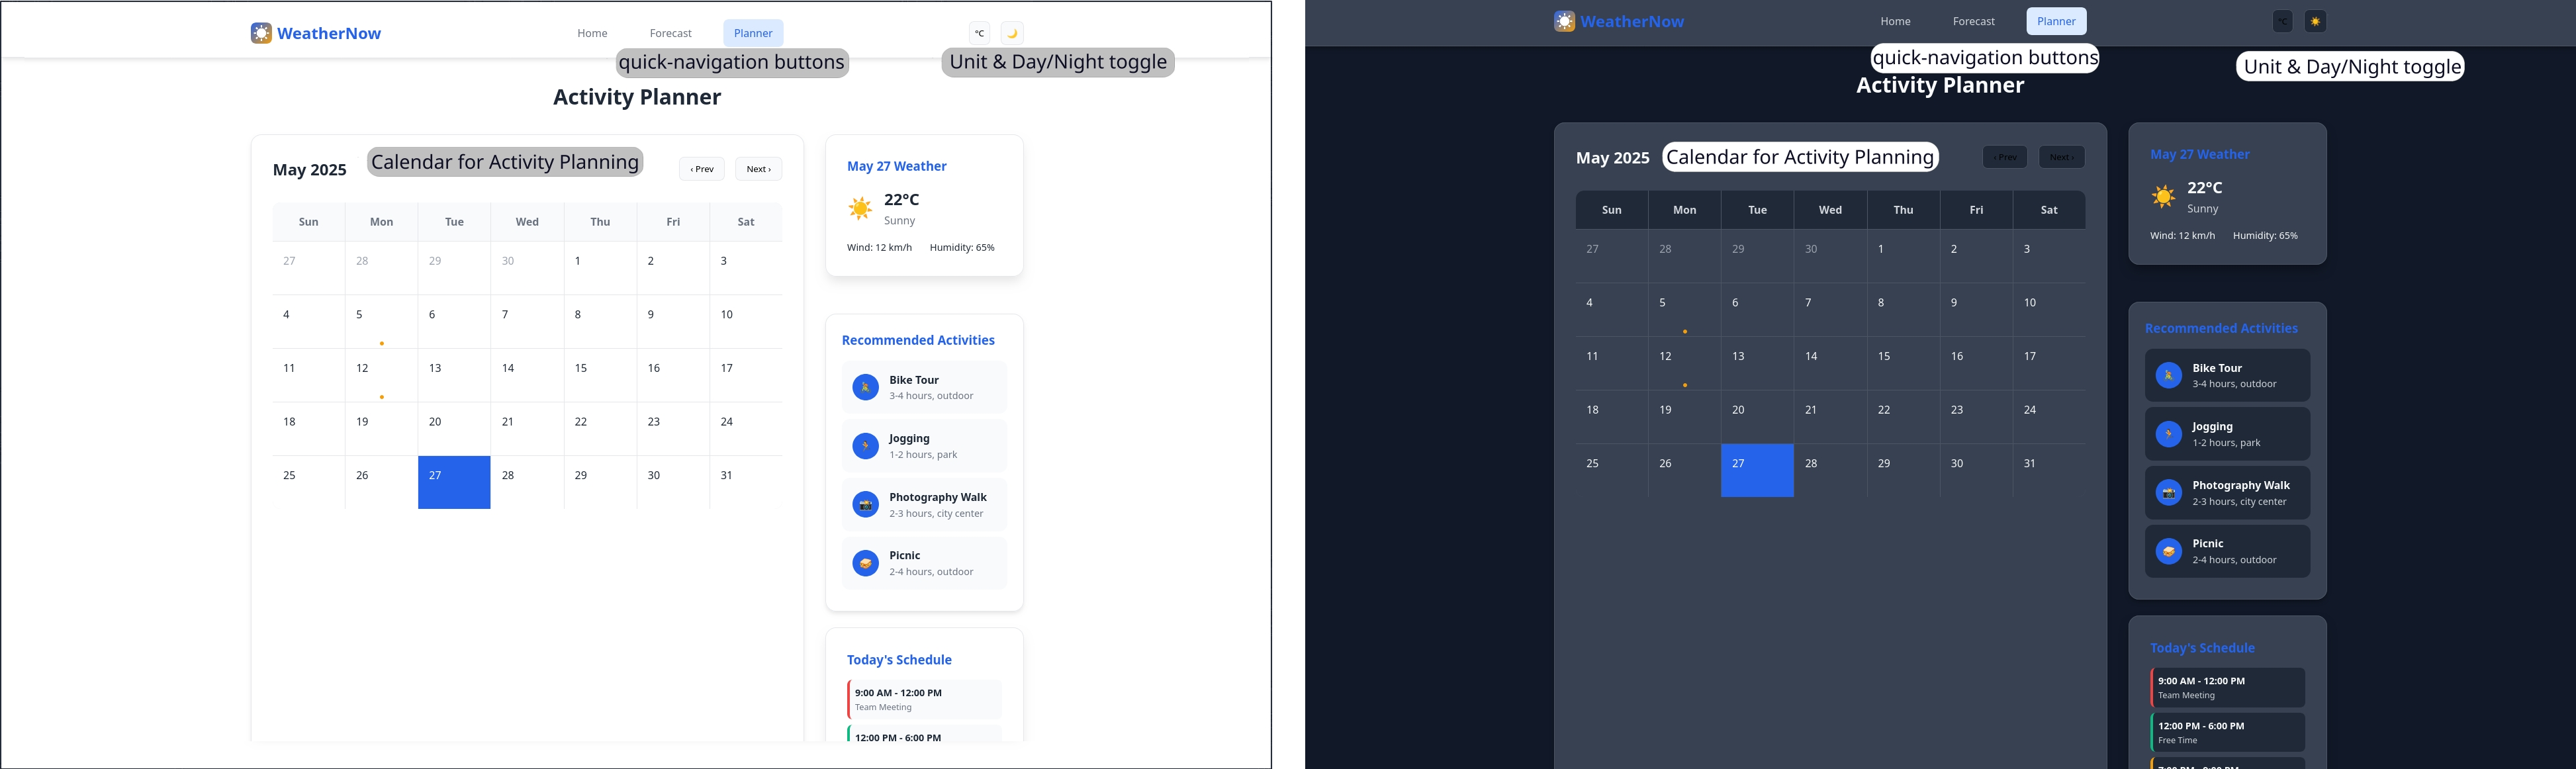
\includegraphics[width=\linewidth]{desktop_planner_descripted.jpg}
  \caption{Calendar view (desktop) showing selectable dates, event slots, weather overlay, and suggested activities.}
  \label{fig:calendar_desktop}
\end{figure}
\FloatBarrier

\subsection{Mobile View}
\FloatBarrier
\begin{figure}[H]
  \centering
  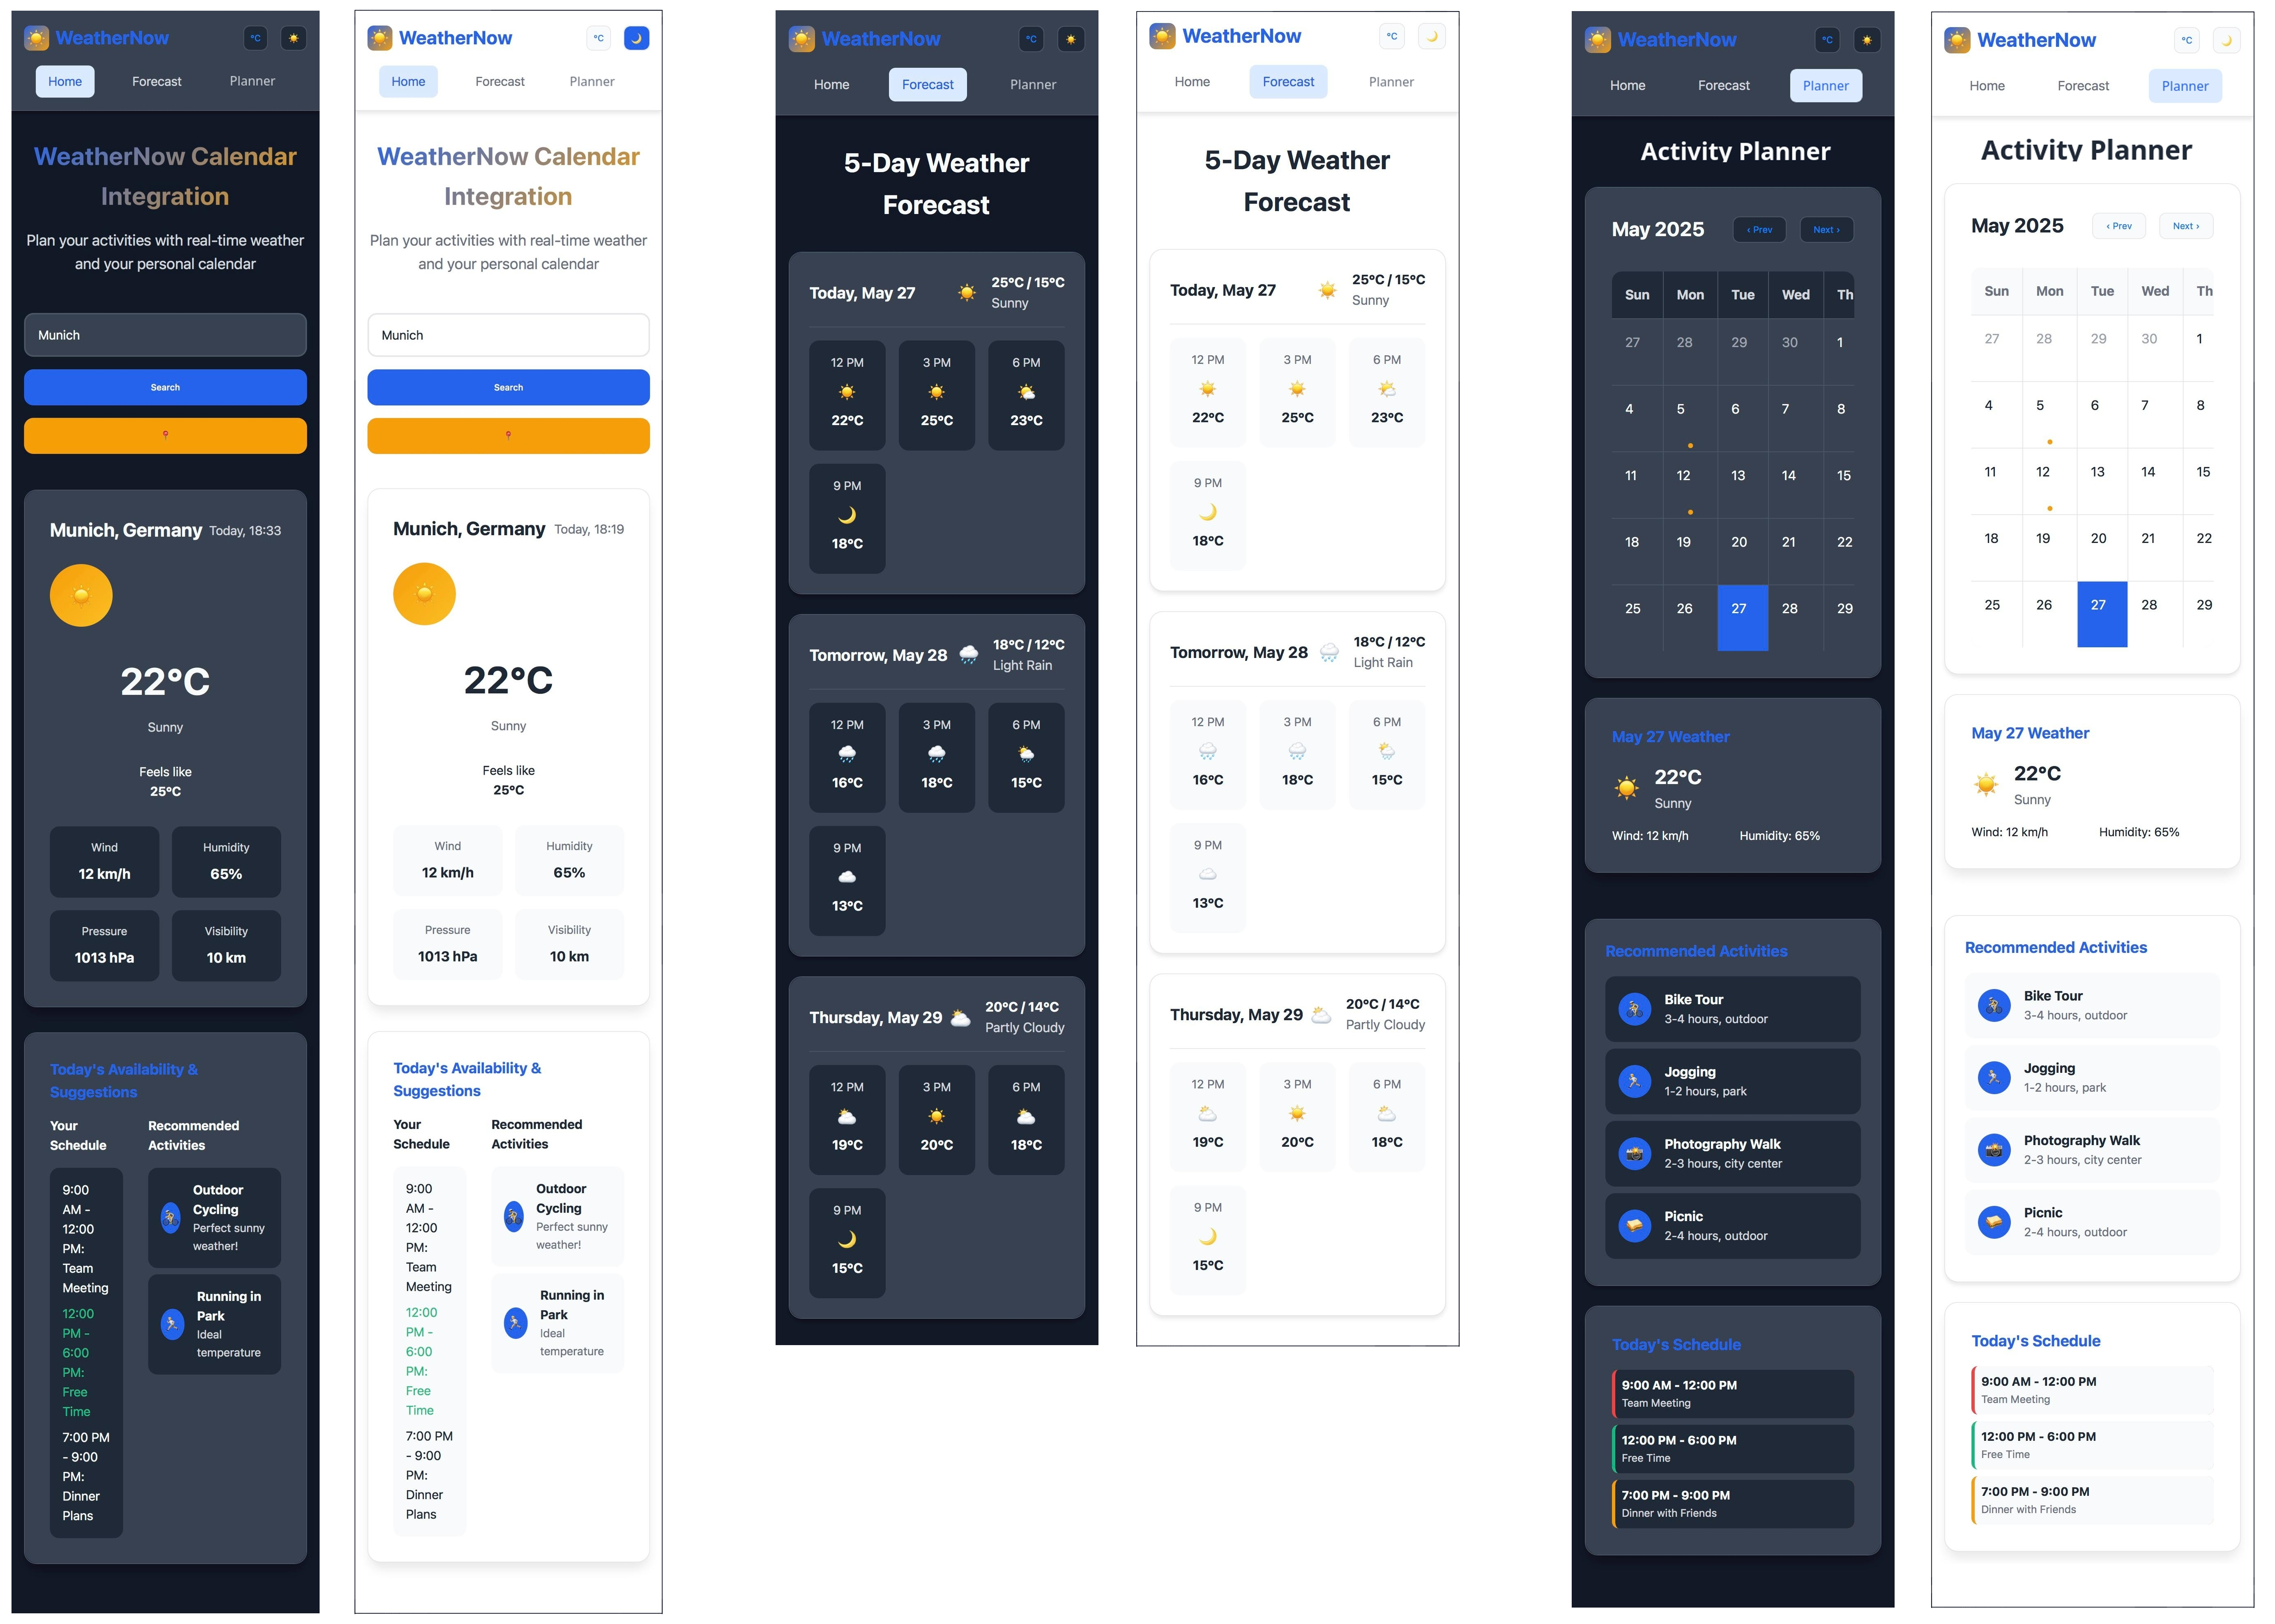
\includegraphics[width=\linewidth]{mobile_all.jpg}
  \caption{Showcase of the mobile implementation with adapted layout}
  \label{fig:calendar_desktop}
\end{figure}
\FloatBarrier

\section{Navigation Flow}
\FloatBarrier
\begin{figure}[H]
  \centering
  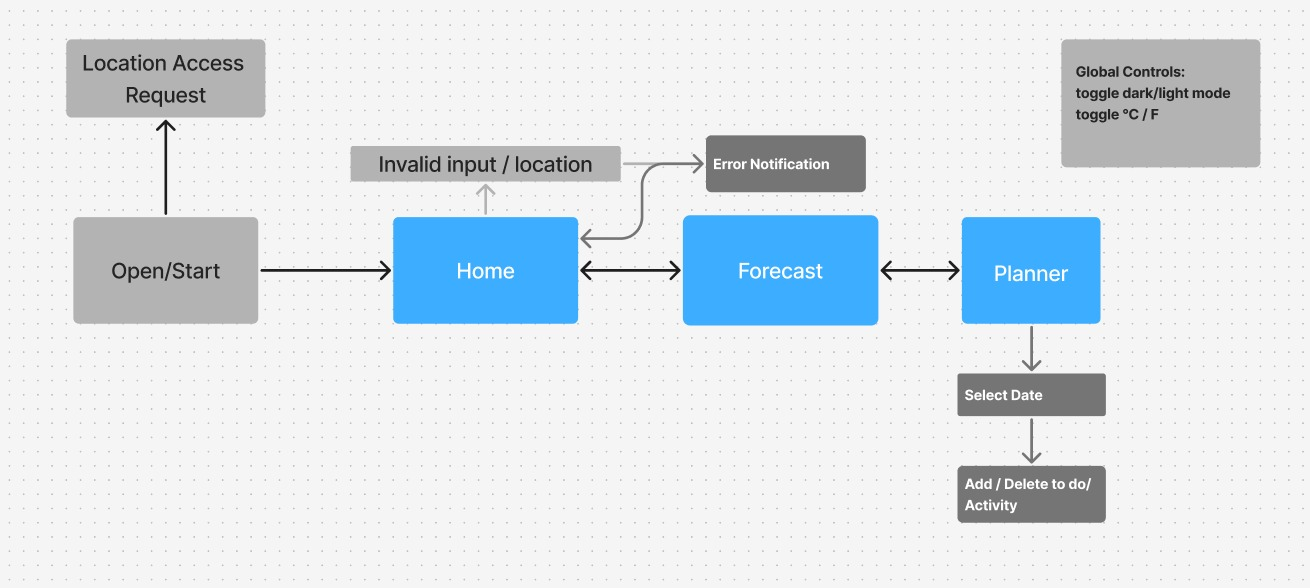
\includegraphics[width=\linewidth]{navigation_flow.jpg}
  \caption{User navigation illustrating consistent, intuitive flow between screens.}
  \label{fig:flow}
\end{figure}
\FloatBarrier

\section{Design Decisions and Rationale}
This section explains the reasoning behind key UI conventions and patterns chosen to meet user needs and requirements.

\subsection{Hierarchy and Layout}
We use a simple and uncluttered header with persistent tabs. In doing so, we ensure users always have Navigation options visible and can quickly switch between Home, Forecast, and Calendar. We want to have the user locate features easily. Information is grouped within card components for weather summaries, forecast intervals, and calendar events. Important info is easy to see at first glance. We intend that users can quickly understand the information, without needing to read everything in detail, therefore being more appealing for busy Professionals and Students (Target User).
\subsection{Theming and Customization}
A light/dark mode toggle respects individual preferences, enhances readability and reduces eye strain. The unit switch (°C/°F) improves usability across different markets and therefore being attractive for example Travelers and Tourists (Target User).
\subsection{Responsive Behavior}
Layouts adapt from a two-column desktop view to a single-column mobile view at breakpoints of 768px and 480px. On mobile, cards are full-width with increased button/input field sizes (minimum 44×44px).

\newpage

\subsection{User Roles/ Use Cases}
This section explains how our design decisions reflect the User Roles and their Use Cases defined in our Requirements Document

\begin{itemize}
  \item US1 Search City: By having the search bar directly easily accessible on the home screen a primary user can quickly enter the desired city and therefore can change between cities with no hassle.
  \item US2 View Forecast: Due to the importance of the forecast to a planner user it has gotten an entire separate tab, which is always accessible from anywhere in the app. Our implementation makes it easy to get an overview of the following days weather to make informed decisions.
  \item US3 grant location access: Like the search bar, the option to grant location access is directly visible in the home tab next(desktop) or below(mobile) the search field. Therefore the action described by the use case is extremely fast, which was a requirement in its implementation.
  \item US4 select date: This Planner use case has been implemented through the calendar integration in the Planner tab. In this section of the website, the user gets information regarding weather, activities and already planned appointments based on the selected date.
  \item US5 toggle Units: This functionality is implemented in the header of the website/mobil app where it is instantly recognizeable and reachable.
  \item US6 toggle theme: Same as the toggle Units button is it easily reachable in the header of the application regardless of the platform.
  \item US7 handle errors:
  \item US8 recent searches: Changing the city to an earlier one is integrated into the search bar itself. when interacting with it, it shows a drop down list with recently input cities and filters these based on the input until now.
  \item US9 severe weather alerts: Warning of severe weather is included in the weather views of both the home and forecast tabs.
  \item US10 multi-language support:
  \item US11 simple layout: This is achieved by splitting the functions into three tabs that each fulfill their given purpose. The home tab as the default tab upon startupacts as a site to quickly get the info for the current situation, the forecast tab as a reference for future planning and the planner tab as a planning screen, that allows structuring ones activities in a simple yet adequate layout.
\end{itemize}

\subsection{Error Handling and Accessibility}
When someone enters a city name wrong, or if there’s a problem with the API, a message pops up right away—either as an alert in the page or as a small notification (toast). This helps users know what’s happening and keeps them confident in the app. All buttons and interactive parts have labels that work with screen readers, and everything can be used with a keyboard. The order of tab through the elements also makes sense. The color choices make sure text is easy to read, following accessibility guidelines.

\section{Responsive behaviour and Accessability Considerations}
The WeatherNow application is built with responsive and accessible design principles for an intuitive experience across devices and for all.

\subsection{Responsive Behavior}
The layout adapts dynamically at key breakpoints (e.g., 768px) as it transitions from multi-column desktop displays to stacked mobile displays. For instance, the calendar reorders from a side-by-side grid to a stacked display, and forecast cards resize to fit smaller screens with fluid grids. Touch targets like tabs and buttons are enlarged on mobile for better usability, and header elements reorganize to maintain clarity and navigation.

\subsection{Accessibility Considerations}
Accessibility is supported by keyboard-navigable controls, high-contrast dark and light themes, and semantic HTML tags. Visual feedback (such as loading spinners and notifications), clear focus states, and logical tab flow keep users informed about system states. While ARIA roles can be added on top, the current structure already supports compatibility with screen readers and assistive software.

\section*{Acknowledgement of AI Technologies}
This document was drafted and refined using GPT-4o based on outlines and reviewed by all authors.

\end{document}
